\documentclass[12pt,oneside,notitlepage,abstracton,a4paper]{scrartcl}
\usepackage{epsfig,scrpage2,graphicx, amsmath, caption, hyperref, natbib, wrapfig, pstricks, epsfig}
\usepackage[font=scriptsize]{subcaption}

\usepackage{listings}
\usepackage{color}

\definecolor{dkgreen}{rgb}{0,0.6,0}
\definecolor{gray}{rgb}{0.5,0.5,0.5}
\definecolor{mauve}{rgb}{0.58,0,0.82}

\lstset{frame=tb,
  language=Python,
  aboveskip=3mm,
  belowskip=3mm,
  showstringspaces=false,
  columns=flexible,
  basicstyle={\small\ttfamily},
  numbers=none,
  numberstyle=\tiny\color{gray},
  keywordstyle=\color{blue},
  commentstyle=\color{dkgreen},
  stringstyle=\color{mauve},
  breaklines=true,
  breakatwhitespace=true,
  tabsize=3
}




\setcounter{secnumdepth}{3}

\setlength{\parindent}{0em}
\setlength{\parskip}{0ex plus0.5ex minus0ex}
\pagestyle{scrheadings}
  

\renewcommand{\headfont}{\normalfont}

\cfoot{\pagemark}

% A picture on top of the titlepage - DESY logo 
\subject{
\includegraphics[scale=0.2]{pics/DESYlogo.pdf}}

\title{\Large X-ray dynamic diffraction of crystalline multilayers and superlattices} 
\author{\normalsize Federica Maria Surace, Scuola Normale Superiore and University of Pisa, Italy}

\date{\normalsize \today}

\begin{document}

\maketitle

\begin{abstract}

\noindent

Numerous methods for the nondestructive characterization of thin epitaxial films,
multilayers and superlattices by x-ray diffraction (XRD) have been developed since the advent of synchrotron radiation sources. In this report, dynamical theory of XRD is used to describe the diffraction profiles of crystalline structures in Bragg case reflection. A software (\textit{dynXRD}) was developed in order to simulate the rocking curves of various types of multilayers and superlattices, including deformed crystals. Results were compared with experimental data, leading to the determination of the strain profile of the sample considered.
\end{abstract}

% If you want, you can also put here a picture %%%


\newpage

% the table of contents is only updated when you run "pdflatex" twice 

\tableofcontents
\newpage 

\section{Introduction}
\label{intro}
The discovery of X-ray diffraction in crystals by Laue, Fridrich and Knipping in 1912 served as the starting point for the development of scientific research along a number of important lines. One of the first and best-known lines of investigation, which advanced rapidly as a result of the discovery, was X-ray analysis of the atomic structure of crystals. The huge amount of experimental data on X-ray structural studies accumulated over more than half century was one of the most important preconditions for developing solid-state physics and chemistry, on the one hand, and the production, processing, and utilization of many materials of contemporary technology, on the other.
\\

Inspired by the result of Fridrich's and Knipping's experiment, Laue devised the simplest theory of three-dimensional diffraction and interference. It was referred to as geometrical or kinematical theory. A characteristics feature of kinematical theory is that it takes into account only the interactions of each atom with the primary, or refracted, wave in a crystal. It neglects the interaction of an atom with the wave field induced in the crystal by the collettive scattering of all the other atoms. In other words it ignores the interaction of the diffracted waves with the refracted one. The kinematical theory is a good first approximation, when applied to highly imperfect crystals consisting of very small mosaic blocks. For the highly perfect type of crystal however, it is necessary to use the more rigorous dynamical theory, and grossly incorrect results would be obtained by using the kinematical approximation.


\section{Dynamical theory of diffraction}
As the incident wave propagates down into a perfect crystal its amplitude diminishes, as a small fraction is reflected into the exit beam as it passes through each atomic plane. In addition there is a chance that the reflected beam will be re-scattered into the direction of the incident beam before it has left the crystal. The theory which has been developed to allow for these multiple scattering effects is known as dynamical diffraction theory.

In the method first developed by C. G. Darwin in 1914, the crystal is treated as an infinite stack of atomic planes, each of which gives rise to a weak reflected wave which may subsequently be re-scattered into the direction of the incident beam.

%Bragg

\subsection{One layer: reflection and transmission}\label{onelayer}

\begin{figure}[h]
\begin{center}
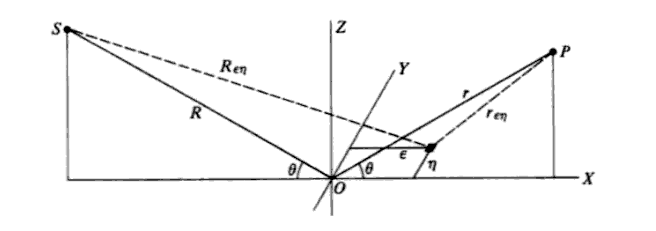
\includegraphics[width=12cm]{pics/picture1.png}
\vspace{-10pt}
\caption{Representation of X-rays from a point source $S$ falling on a layer in the $XY$-plane near the Bragg condition. Scattered radiation is observed at the point $P$. For the origin $O$, the path length $R+r$ is a minimum.}
\label{pic1}
\vspace{-10pt}
\end{center}
\end{figure}

We consider first the reflection from a single layer of the crystal near the Bragg case. Let the incident beam be $\sigma$-polarized (i.e. the electric field is parallel to the layer) and have a wavelength $\lambda$. We can calculate the amplitude of the reflected and transmitted beams by considering the radiation scattered from an element of area $d\epsilon d\eta$ and integrating over the layer. We obtain the following expression for the instantaneous value of the electric field at point $P$ (figure \ref{pic1})

\begin{equation}
 E_P=-ig_\mathbf{H}E_Oe^{(2\pi i /\lambda)[(R+r)-ct]}.
\end{equation}

We introduced the abbreviation

\begin{equation}\label{eqg}
 g_\mathbf{H}=r_e\frac{\lambda F_\mathbf{H}d}{V \sin{\theta_B}}
\end{equation}

where $r_e=\frac{e^2}{mc^2}=2.818 \cdot 10^{-5} \AA{}$ is the classical electron radius, $F_\mathbf{H}$ is the structure factor for the reciprocal lattice vector $\mathbf{H}$, $d$ is the spacing of the reflecting planes, $V$ is the volume of the unit cell and $\theta_B$ is the Bragg angle.

\begin{figure}[h]
\begin{center}
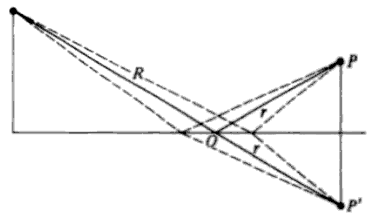
\includegraphics[width=7cm]{pics/picture2.png}
\vspace{-10pt}
\caption{For the scattering by the atoms in a plane, the path lengths are the same for a point $P$ and its mirror image $P'$.}
\label{pic2}
\vspace{-10pt}
\end{center}
\end{figure}


Similarly, the electric field in the beam which has passed through a layer of unit cells (figure \ref{pic2}) is expressed by
\begin{equation}\label{Et}
 E_{P'}=(1-ig_0)E_Oe^{(2\pi i /\lambda)[(R+r)-ct]}
\end{equation}

where
\begin{equation} \label{eqg0}
 g_0=r_e\frac{\lambda F_0 d}{V \sin{\theta_B}}.
\end{equation}

Since $V$ is of order $d^3$, $g_\mathbf{H}$ and $g_0$ are of order $r_0/d \simeq 10^{-5} \ll 1$.

\newpage
\subsection{Diffraction from a set of planes}
\begin{wrapfigure}{r}{0.4\textwidth}
\vspace{-40pt}
\begin{center}
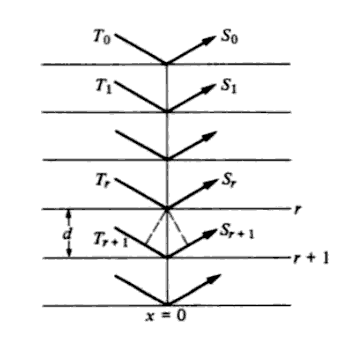
\includegraphics[width=7cm]{pics/picture3.png}
\caption{Diffraction from a set of atomic planes.}
\label{pic3}
\end{center}
\end{wrapfigure}We now turn our attention to the problem of how to calculate the scattering from an infinite stack of atomic planes, where each one reflects and transmits the incident wave according to the equations given in section \ref{onelayer}. The planes are labelled by the index $r$, with the surface plane defined by $r=0$. The objective is to calculate the amplitude reflectivity, which is the ratio of the total reflected wavefield $S_0$ to that of the incident field $T_0$.

Both outside and within the crystal there are two wavefields: the $T$ field propagating in the direction of the incident beam , and the $S$ field in the direction of the reflected beam (figure \ref{pic3}).




The derivation of Bragg's law relies on the fact that the reflected wave from layer $r+1$ is in phase with the one from layer $r$ if the pathlength differs by an integer number of wavelengths (equation \ref{bragg}). 
\begin{equation}\label{bragg}
 2\sin{\theta_B}=m\lambda
\end{equation}

As we are interested in deriving the (small) bandwidth of the reflecting region, the phase is restricted to small deviations about $m\pi$, and the phase is given by
\begin{equation}\label{phase}
 \phi=m\pi+\Delta
\end{equation}
where $\Delta$ is a small parameter. In our development of Darwin's theory $\Delta$ will be used as the independent variable.

Let the $T$ field just above layer $r$ on the $z$ axis be denoted $T_r$, and similarly for $S_r$. On being transmitted through the $r$th layer, the $S$ field just above layer $r+1$ changes its phase according to equation \ref{Et}, so that $S_r$ can be written as $(1-ig_0)S_{r+1}e^{i\phi}$. To obtain the total field, we must also add the part due to the reflection of the wave $T_r$. In total then we have
\begin{equation}\label{eq:TS1}
 S_r=-ig_\mathbf{H}T_r+(1-ig_0)S_{r+1}e^{i\phi}
\end{equation}

Next consider the $T$ field just below the $r$th layer. The phase is shifted by $\phi$. This field is composed of contributions from the field $T_r$ after it has been transmitted through the $r$th layer, and from the wave $S_{r+1}e^{i\phi}$ after it has been reflected from the bottom of the $r$th layer. This leads to the second difference equation
\begin{equation}\label{eq:TS2}
 T_{r+1}e^{-i\phi}=(1-ig_0)T_r-ig_\mathbf{\bar{H}}S_{r+1}e^{i\phi}
\end{equation}

A suitable trial solution for \ref{eq:TS1} and \ref{eq:TS2} including a phase shift and attenuation has the form
\begin{equation}
T_{r+1}=e^{-\chi}e^{im\pi}T_r, \quad
S_{r+1}=e^{-\chi}e^{im\pi}S_r
\end{equation}
where $\chi$ is a general complex. We can now insert our trial solution into the equations. Noting that $e^{-i\phi}=e^{-im\pi}e^{-i\Delta}$ and expanding all the small parameters to second-order terms yields

\begin{equation}
\chi^2=g_\mathbf{H}g_\mathbf{\bar{H}}-(\Delta-g_0)^2
\end{equation}
which has the solution
\begin{equation}
i\chi=\pm \sqrt{(\Delta-g_0)^2-g_\mathbf{H}g_\mathbf{\bar{H}}}.
\end{equation}

We can now calculate the amplitude reflectivity by inserting our solutions into equation \ref{eq:TS1}. Let $g$ be equal to $\sqrt{g_\mathbf{H}g_\mathbf{\bar{H}}}$. We obtain
\begin{equation}\label{eq:r}
X_R=\frac{S_0}{T_0} \simeq \frac{g}{i\chi+(\Delta-g_0)}
\end{equation}
In order to obtain explicit formulae for the Darwin reflectivity curve the variable $\eta$ is introduced and defined by
\begin{equation}
\eta=\frac{\Delta-g_0}{g}.
\end{equation}
From equation \ref{eq:r} the amplitude reflectivity curve in terms of $\eta$ is
\begin{equation}\label{eq:darwin}
 X_R=\frac{S_0}{T_0}=
 \begin{cases}
  \eta-\sqrt{\eta^2-1} & \quad \text{for } \eta\ge 1  \\
  \eta-i\sqrt{1-\eta^2} & \quad \text{for } |\eta|\le 1  \\
  \eta+\sqrt{\eta^2-1} & \quad \text{for } \eta\le -1  \\
 \end{cases}
\end{equation}


%picture

\subsection{General case: substrate}
%picture

\begin{wrapfigure}{l}{0.5\textwidth}
\begin{center}
\vspace{-20pt}
\scalebox{0.8} % Change this value to rescale the drawing.
{
\begin{pspicture}(-4,-1.5)(4,4)
\psline[linewidth=0.04cm,arrowsize=0.08cm 2.0,arrowlength=1.4,arrowinset=0.4]{->}(0,0)(3,2)
\psline[linewidth=0.04cm,arrowsize=0.08cm 2.0,arrowlength=1.4,arrowinset=0.4]{->}(-3,2)(0,0)
\psline[linewidth=0.04cm,arrowsize=0.08cm 2.0,arrowlength=1.4,arrowinset=0.4,linestyle=dashed,dash=0.16cm 0.16cm]{->}(0,0)(0,4)
\psline[linewidth=0.04cm,arrowsize=0.08cm 2.0,arrowlength=1.4,arrowinset=0.4]{->}(-2,-0.8)(1,1.2)
\psline[linewidth=0.04cm,arrowsize=0.08cm 2.0,arrowlength=1.4,arrowinset=0.4]{->}(-5,1.2)(-2,-0.8)
\psline[linewidth=0.04cm,arrowsize=0.08cm 2.0,arrowlength=1.4,arrowinset=0.4]{<->}(-1.615,1.077)(-2.6,-0.4)
\psline[linewidth=0.04cm,arrowsize=0.08cm 2.0,arrowlength=1.4,arrowinset=0.4]{<->}(0.354,0.769)(0.6,0.4)
\psline[linewidth=0.04cm,arrowsize=0.08cm 2.0,arrowlength=1.4,arrowinset=0.4,linestyle=dashed,dash=0.16cm 0.16cm]{->}(0,0)(-0.8,2)
\psline[linewidth=0.04cm](-4,-1.6)(4,1.6)
\psline[linewidth=0.04cm](-4,-1.6)(4,-1.6)
\psline[linewidth=0.04cm](-0,0)(4,0)
\psline[linewidth=0.04cm](-2,-0.8)(4,-0.8)
\psline[linewidth=0.04cm](2,0.8)(4,0.8)
\psline[linewidth=0.04cm](-1,-0.4)(4,-0.4)
\psline[linewidth=0.04cm](1,0.4)(4,0.4)
\psline[linewidth=0.04cm](-3,-1.2)(4,-1.2)
\psline[linewidth=0.04cm](3,1.2)(4,1.2)
\rput(-1.5,1.5){$\mathbf{k_{in}}$}
\rput(1.5,1.5){$\mathbf{k_{out}}$}
\rput(0.2,2){$\mathbf{q}$}
\rput(-0.6,2.1){$\mathbf{n}$}
\end{pspicture} 
}
\caption{Asymmetric Bragg reflection. The widths of the incident and scattered beams are different.}
\label{asymmpic}
\end{center}
\end{wrapfigure}


In general the surface of the crystal will not be parallel to the atomic planes which reflect the incident beam, as shown in picture \ref{asymmpic}. This implies a compression of the width of the exit beam. The asymmetry parameter $b$ is defined as
\begin{equation}\label{bdef}
 b=\frac{\gamma_0}{\gamma_\mathbf{H}}
\end{equation}
where $\gamma_0$ is the cosine of the angle between the incident beam and the surface normal and $\gamma_H$ is the cosine of the angle between the diffracted beam and the surface normal (equation \ref{gamma}; in the Bragg case $b$ is always negative).
\begin{equation}\label{gamma}
\gamma_0=\frac{\mathbf{k_{in}}\cdot \hat{n}}{|\mathbf{k_{in}}|},\quad \gamma_\mathbf{H}=\frac{\mathbf{k_{out}}\cdot \hat{n}}{|\mathbf{k_{out}}|}
\end{equation}


Equation \ref{eq:darwin} is still valid in the asymmetric case if we include the asymmetric parameter in the variable $\eta$ as follows
\begin{equation}\label{asymm}
 \eta=\frac{-b\Delta-g_0(1-b)/2}{|b|^{1/2}g}
\end{equation}

From equations \ref{bragg} and \ref{phase} and using the fact that $\Delta$ is small we obtain
\begin{equation}\label{Delta}
 \Delta=\frac{2\cos{\theta_B} \pi d}{\lambda}(\theta-\theta_B)
\end{equation}
Substitution of the expressions \ref{eqg}, \ref{eqg0} and \ref{Delta} into equation \ref{asymm} leads to a new expression for $\eta$
\begin{equation}\label{eta}
 \eta=\frac{-b(\theta-\theta_B) \sin{2 \theta_B}-\frac{1}{2}\Gamma F_0(1-b)}{|b|^{1/2}C\Gamma(F_\mathbf{H}F_\mathbf{\bar{H}})}.
\end{equation}


\subsection{General case: epitaxial layer}
In a similar way it is also possible to use dynamical theory to calculate the reflected and transmitted amplitude ratios ($X_R$ and $X_T$) for layers of arbitrary thickness $t$. For convenience we introduce the parameters
\begin{equation}
 T=\pi \Gamma (F_\mathbf{H}F_\mathbf{\bar{H}})^{1/2}\frac{t}{\lambda |\gamma_0 \gamma_\mathbf{H}|^{1/2}}
 \end{equation}
\begin{equation}
 \alpha=T(\eta^2-1)^{1/2}
 \end{equation}
\begin{equation}
 Q=(\eta^2-1)^{1/2}\cos{\alpha} +i\eta \sin{\alpha}.
\end{equation}
where $\eta$ is the variable we defined in equation \ref{eta}.

The equations for $X_R$ and $X_T$ reduce to
\begin{equation}\label{XR}
 X_R=\frac{i \sin{\alpha}}{Q}
 \end{equation}
\begin{equation}\label{XT}
 X_T=\frac{(\eta^2-1)^{1/2}}{Q}.
\end{equation}

The absolute squares of $X_R$ and $X_T$ are the reflectivity (figure \ref{dyn}) and transmittivity of the layer.

\begin{figure}[h]
\begin{center}
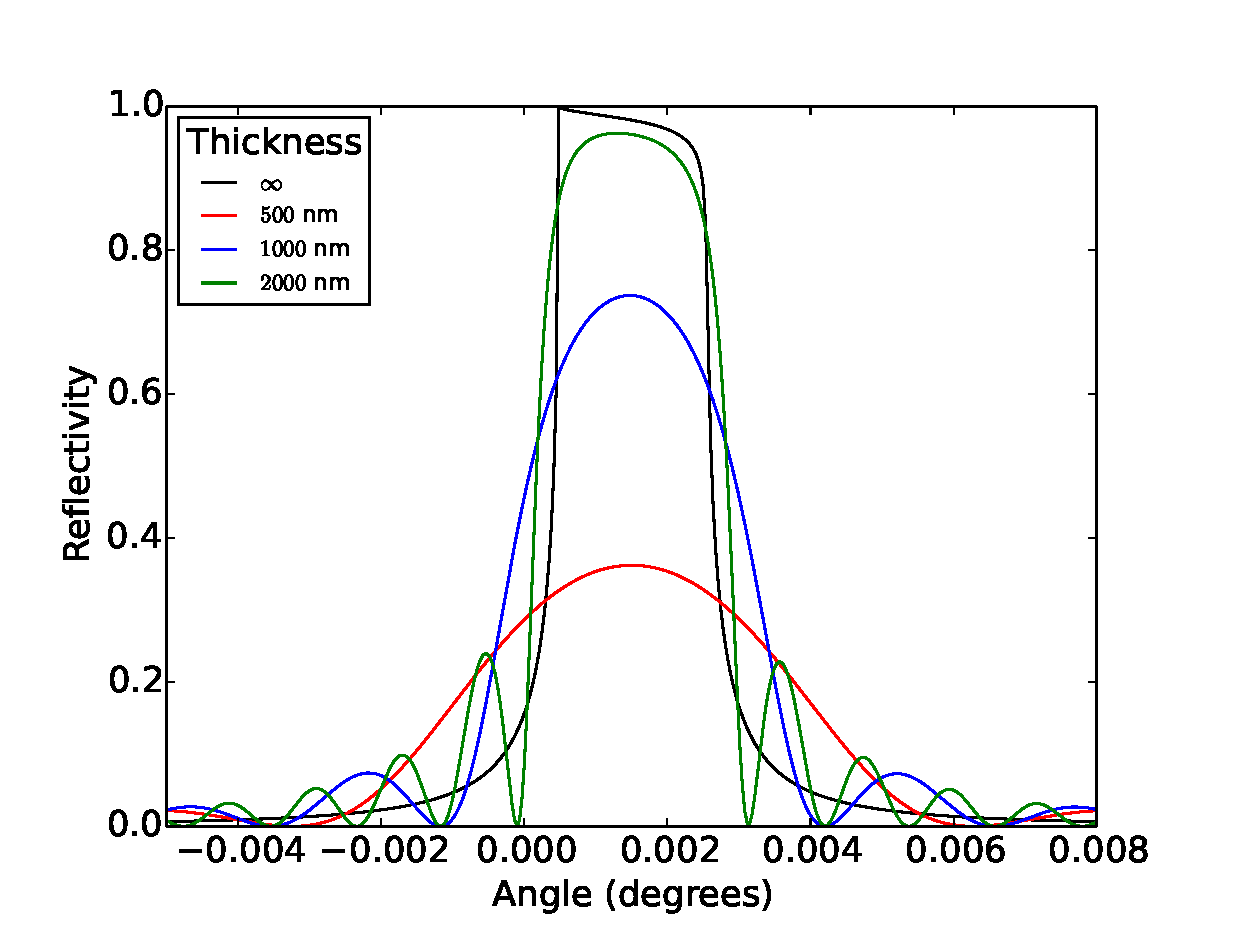
\includegraphics[width=12 cm]{pics/dynamical.eps}
\caption{Darwin curve of a MgO $002$ reflection. If X-ray absorption were absent, the top of the curve of the infinitely thick crystal would be flat (Darwin plateau).}
\label{dyn}
\end{center}
\end{figure}


\newpage
\subsection{Recursion formulae}
When an epitaxial layer with reflected and transmitted amplitude ratios $X_R^1$ and $X_T^1$ is added to a substrate with ratios $X_R^0$, $X_T^0$, the new amplitude ratios $X_t$, $W$ for the crystal can be derived in a recursive way. In combining the crystal parts in figure \ref{rec}, the incident beam of the lower part is replaced by the transmitted beam of the upper part.
\begin{figure}[h]
\begin{center}
\scalebox{1}
{
\begin{pspicture}(0,0)(4,3)
\psframe[linewidth=0.04,dimen=outer](0,1)(4,1.2)
\psline[linewidth=0.04cm,arrowsize=0.06cm 2.0,arrowlength=1.4,arrowinset=0.4]{->}(1.3,2.9)(1.9,2.3)
\psline[linewidth=0.04cm,arrowsize=0.06cm 2.0,arrowlength=1.4,arrowinset=0.4]{->}(1.3,1.9)(1.9,1.3)
\psframe[linewidth=0.04,dimen=outer](0,2)(4,2.2)
\psline[linewidth=0.04cm,arrowsize=0.06cm 2.0,arrowlength=1.4,arrowinset=0.4]{->}(2.1,2.3)(2.7,2.9)
\psline[linewidth=0.04cm,arrowsize=0.06cm 2.0,arrowlength=1.4,arrowinset=0.4]{->}(2.1,1.3)(2.7,1.9)
\psline[linewidth=0.04cm,arrowsize=0.06cm 2.0,arrowlength=1.4,arrowinset=0.4]{->}(1.6,0.9)(2.2,0.3)
%\usefont{T1}{ptm}{m}{n}
\rput(2.9,2.6){$X_t$}
%\usefont{T1}{ptm}{m}{n}
\rput(1.1,1.6){$Z$}
%\usefont{T1}{ptm}{m}{n}
\rput(2.9,1.6){$Y$}
%\usefont{T1}{ptm}{m}{n}
\rput(2.4,0.6){$W$}
\rput(4.9,2.1){$X_R^1$, $X_T^1$}
\rput(4.9,1.1){$X_R^0$, $X_T^0$}
\end{pspicture} 
}
\caption{In the recursion process a thin layer of thickness $t$ is added to the previous layer so that the reflected and transmitted amplitude ratios at the surface change from $X_R^0$, $X_T^0$ to $X_t$, $W$.}
\label{rec}
\end{center}
\end{figure}



Owing to multiple reflections the amplitude ratios will vary but can be expressed in the original values $X_R^0$, $X_T^0$, $X_R^1$ and $X_T^1$, so that
\begin{equation}
 X_t=X_T^1 Y+X_R^1
\end{equation}
\begin{equation}
 Z=X_R^1 Y+X_T^1
\end{equation}
\begin{equation}
 Y=X_R^0 Z
\end{equation}
\begin{equation}
 W=X_T^0 Z.
\end{equation}

After substitution, we obtain the reflected and transmitted amplitude ratios for the sample
\begin{equation}\label{refl}
 X_t=\frac{X_R^1-X_R^0({X_R^1}^2-{X_T^1}^2)}{1-X_R^0 X_R^1}
\end{equation}
\begin{equation}\label{trans}
 W=\frac{X_T^0 X_T^1}{1-X_R^0 X_R^1}.
\end{equation}





\section{Implementation}

In order to simulate the rocking curves of strained crystals, multilayers and superlattices in the dynamical theory, a Python program has been developed. The program \textit{dynXRD} is applicable to any coplanar and non-coplanar Bragg-case geometry (see section \ref{geom}) and to crystals with any number of different layers. Layers with arbitrary strain profile are also implemented (see section \ref{strcr}). At the moment perpendicular ($\sigma$) polarization is the only one enabled, but parallel ($\pi$) and mixed polarizations may be included in the future. The program requires \textit{pyasf} () for the definition of the crystal structure and for the calculation of the structure factors.

%something about pyasf

\subsection{Structure}
The program calculates the reflected and transmitted amplitude ratios for an instance object of the class \textit{Sample}. A \textit{Sample} object is nothing but a sequence of other objects of the class \textit{Epitaxial\_Layer}.

For each \textit{Epitaxial\_Layer} the following attributes have to be given:
\begin{itemize}
 \item \textbf{structure} of the crystal, which is taken from a \textit{.cif} file
 \item \textbf{thickness} of the layer in Angstrom
 \item \textbf{R} matrix, i.e. a rotation matrix containing information about the orientation of the unit cell with respect to the surface of the sample
 \item \textbf{Miller} indices of the considered Bragg reflection.
\end{itemize}

A special type of \textit{Epitaxial\_Layer} is defined by the class \textit{Substrate}. The thickness of a \textit{Substrate} is set to be infinity and the transmitted amplitude is zero. A \textit{Sample} is then made of a \textit{Substrate} object and a list of \textit{Epitaxial\_Layer} objects.

Once the Miller indices (with respect to the substrate) are given by the user through the method \textit{Sample.set\_Miller}, the program calculates the $\mathbf{q}$ vector in the sample system by using rotation matrices. The Miller indices with respect to a layer are then obtained as the integers which best approximate the coordinates of the $\mathbf{q}$ vector in the reciprocal lattice system of the crystal. As a result we get the reciprocal space vector which corresponds to the Bragg case for the layer. The expressions for the angles between the incident beam and these vectors are then calculated with the method \textit{Sample.calc\_theta\_layer}. After evaluation of these expressions we get the angle $\theta$ to insert in equation \ref{eta}.

%code?
%calc of XR and XT

\subsection{Geometrical parameters}\label{geom}

%picture!
The geometry of each crystal layer is needed in order to calculate the change in the angle $\theta$ and the quantities $\gamma_0$ and $\gamma_\mathbf{H}$ that we used to define the asymmetry parameter $b$ (equation \ref{bdef}).


\begin{figure}[h]
\begin{center}
\scalebox{1} % Change this value to rescale the drawing.
{
\begin{pspicture}(-3,-2)(3,4)
\pspolygon[linewidth=0.04](-3,0)(3,0)(1.8,-1.6)(-4.2,-1.6)
\pspolygon[linewidth=0.04](-3,0)(3,0)(3.8,3.6)(-2.2,3.6)
\psline[linewidth=0.04cm](3,0)(4.2,1.6)
\psline[linewidth=0.04cm](3.35,1.6)(4.2,1.6)
\psline[linewidth=0.04cm,arrowsize=0.06cm 2.0,arrowlength=1.4,arrowinset=0.4]{->}(-0.75,1.75)(0,0)
\psline[linewidth=0.04cm,arrowsize=0.06cm 2.0,arrowlength=1.4,arrowinset=0.4]{->}(0,0)(1.95,0.95)
\psline[linewidth=0.04cm,arrowsize=0.06cm 2.0,arrowlength=1.4,arrowinset=0.4]{->}(0,0)(1.2,2.7)
\psline[linewidth=0.04cm,arrowsize=0.06cm 2.0,arrowlength=1.4,arrowinset=0.4, linestyle=dashed,dash=0.1cm 0.1cm]{->}(0,0)(0,1.5)
\psline[linewidth=0.04cm, linestyle=dashed,dash=0.06cm 0.06cm](0.6,-2)(-1.2,-1.6)
\psline[linewidth=0.04cm, linestyle=dashed,dash=0.06cm 0.06cm](-0.4,-2)(-2.2,-1.6)
\psline[linewidth=0.04cm, linestyle=dashed,dash=0.06cm 0.06cm](-1.4,-2)(-3.2,-1.6)
\psline[linewidth=0.04cm, linestyle=dashed,dash=0.06cm 0.06cm](-2.4,-2)(-4.2,-1.6)
\psline[linewidth=0.04cm, linestyle=dashed,dash=0.06cm 0.06cm](1.6,-2)(-0.2,-1.6)
\psline[linewidth=0.04cm, linestyle=dashed,dash=0.06cm 0.06cm](2.6,-2)(0.8,-1.6)
\psline[linewidth=0.04cm, linestyle=dashed,dash=0.06cm 0.06cm](3.6,-2)(1.8,-1.6)
\psline[linewidth=0.04cm,arrowsize=0.06cm 2.0,arrowlength=1.4,arrowinset=0.4]{->}(5,0)(6.5,0)
\psline[linewidth=0.04cm,arrowsize=0.06cm 2.0,arrowlength=1.4,arrowinset=0.4]{->}(5,0)(5,1.5)
\psline[linewidth=0.04cm,arrowsize=0.06cm 2.0,arrowlength=1.4,arrowinset=0.4]{->}(5,0)(5.9,1.2)
\psarc[linewidth=0.04](0.05,0.15){0.37}{13}{127}
\rput(-0.65,0.7){$\mathbf{k_{in}}$}
\rput(1.8,0.5){$\mathbf{k_{out}}$}
\rput(0.95,1.5){$\mathbf{q}$}
\rput(0.15,1.7){$\hat{n}$}
\rput(6.7,0){$\hat{x}$}
\rput(5.9,0.8){$\hat{y}$}
\rput(4.7,0.5){$\hat{z}$}
\rput(0.5,0.5){$\theta$}
\rput(-0,0.7){$\theta$}
\end{pspicture} 
}
\caption{Asymmetric reflection in non-coplanar geometry.}
\label{geom2}
\end{center}
\end{figure}


Let $\mathbf{a}$, $\mathbf{b}$ and $\mathbf{c}$ be the lattice vector and $\mathbf{a^*}$, $\mathbf{b^*}$ and $\mathbf{c^*}$ the reciprocal lattice vectors.
Let $\hat{x}$, $\hat{y}$ and $\hat{z}$ be the unit vectors of the sample system, such that the normal to the sample surface $\hat{n}$ is parallel to $\hat{z}$ and that $\hat{x}$ lies on the scattering plane.
The geometry of the crystal layers can be specified in 2 different ways.
With the method \textit{Epitaxial\_Layer.calc\_orientation} the user can set the coordinates in the reciprocal lattice system of two vectors $\mathbf{v_\perp}$ and $\mathbf{v_\parallel}$ which are respectively parallel to $\hat{z}$ and $\hat{x}$. The two vectors given should be perpendicular by definition. If this is not the case an error message is printed. To prevent this, the method \textit{Epitaxial\_Layer.calc\_orientation\_from\_angle} was developed: the user can give as input an angle $\psi$, which is the angle between $\mathbf{v_\parallel}$ and a reference vector $\mathbf{p}$. The vector $\mathbf{p}$ is defined as the vector perpendicular to $\mathbf{b^*}$ and $\mathbf{v_\perp}$:
\begin{equation}
 \mathbf{p}=\mathbf{b^*} \times \mathbf{v_\perp}.
\end{equation}
If $\mathbf{b^*}$ and $\mathbf{v_\perp}$ are parallel then $\mathbf{p}$ is defined as
\begin{equation}
 \mathbf{p}=\mathbf{v_\perp} \times \mathbf{c^*}
\end{equation}



\begin{wrapfigure}{r}{0.3\textwidth}
\begin{center}
\vspace{-10pt}
\scalebox{1} % Change this value to rescale the drawing.
{
\begin{pspicture}(0,0)(4.5,2.6)
\pspolygon[linewidth=0.04](0.0,0)(3.5,0)(4.5,2)(1,2)
\psline[linewidth=0.04cm,arrowsize=0.06cm 2.0,arrowlength=1.4,arrowinset=0.4]{->}(2,1)(2,2.6)
\psline[linewidth=0.04cm,arrowsize=0.06cm 2.0,arrowlength=1.4,arrowinset=0.4]{->}(2,1)(3.15,1.65)
\psline[linewidth=0.04cm,arrowsize=0.06cm 2.0,arrowlength=1.4,arrowinset=0.4]{->}(2,1)(3.3,0.9)
\psarc[linewidth=0.04](2.5, 1.1){0.24}{320}{75.0}
\rput(1.7,1.5){$\mathbf{v_\perp}$}
\rput(2.6,1.6){$\mathbf{p}$}
\rput(2.8,0.6){$\mathbf{v_\parallel}$}
\rput(3,1.2){$\psi$}
\end{pspicture} 
}
\caption{Geometrical characterization of the Bragg reflection.}
\vspace{-10pt}
\label{geom1}
\end{center}
\end{wrapfigure}

Specification of $\mathbf{v_\parallel}$ is no longer required since it can be calculated from $\psi$. Now $\mathbf{v_\parallel}$ is automatically perpendicular to $\mathbf{v_\perp}$ and no errors occur.

The vector $\mathbf{v_\perp}$ and $\mathbf{v_\parallel}$ specify the geometry of the reflection.
If $\mathbf{v_\perp}$ and $\mathbf{H}$ are parallel - i.e. if the asymmetry factor $b$ is equal to $-1$ - the reflection is \textit{symmetric}. If this condition is not fulfilled the reflection is said to be \textit{asymmetric}.
We call the geometry \textit{coplanar} when the incident wave vector $\mathbf{k_{in}}$, the reciprocal lattice vector $\mathbf{H}$, and the surface normal $\mathbf{n}$ lie in the same plane or equivalently when $\mathbf{v_\parallel}$, $\mathbf{v_\perp}$ and $\mathbf{H}$ are coplanar.

%details?
%code?
%something about M and R?


\subsection{Reflectivity}
Calculation of reflected and transmitted amplitudes of a layer is implemented via the methods \textit{Epitaxial\_Layer.calc\_parameters} and \textit{Epitaxial\_Layer.calc\_amplitudes} which apply equations \ref{eq:darwin} (for the substrate), \ref{XR} and \ref{XT} (for the epitaxial layers).

After solving the dynamical diffraction problem for each layer, the reflection from the whole stack is calculated with equation \ref{refl}:
\begin{lstlisting}
    def calc_reflectivity(self, theta, Energy, Polarization=1):
        self.calc_theta_layer()
        self.calc_g0_gH(Energy)
        self.substrate.calc_amplitudes(theta, Energy)
        X0=self.substrate.XR
        for layer in self.Layers:
            layer.calc_amplitudes(theta, Energy)
            XR=layer.XR
            XT=layer.XT
            Xt=(XR-X0*(XR**2-XT**2))/(1-X0*XR)
            X0=Xt
        return X0
\end{lstlisting}


\subsection{Strained crystals} \label{strcr}
The recursion formulae (\ref{refl}) and (\ref{trans}) can be used for samples made of different epitaxial layers, but also hold for a single crystal with a given strain profile. The strained crystal is treated as a stack of layers with constant strain. To do so a new class of \textit{Epitaxial\_Layer} was defined. An instance of a \textit{Strained\_Layer} requires two arrays of the same length: an array containing the depths (distances from the substrate surface) and an array containing the strain of a lattice parameter (for example $\frac{\Delta a}{a}$) at different depths.

The amplitudes of reflected and transmitted beams are calculated for each sublayer with constant strain by substituting the value of the modified lattice parameter in the expressions and using equations \ref{XR} and \ref{XT}. The total amplitudes of the layer are then obtained by iterating the formulas \ref{refl} and \ref{trans} through all sublayers.

%code?

%print values


\section{Results}

The program \textit{dynXRD} was first tested by comparing the results with the program \textit{GID\_sl} created by Sergey Stepanov (\url{http://x-server.gmca.aps.anl.gov/GID_sl.html}). Some examples are reported in sections \ref{res1} and \ref{res2}. Results for strained layers also match with the rocking curves calculated by Bartels, Hornstra and Lobeek \cite{Bartels:a25435} (figure \ref{GaAs_both}). In section \ref{data} simulation and experimental data are compared in order to get information about the strain profile of the sample.


\subsection{Rocking curves of crystalline multilayers}\label{res1}
Figures \ref{testsMgO} and \ref{testsLiNbO3} show the simulated rocking curves of crystalline layers (cubic MgO and trigonal LiNbO$ _3$) of thickness $100\;nm$ when an incident beam of energy $10\; keV$ is applied. 

\begin{figure}[h]
 \centering
 \begin{subfigure}[h]{0.49\textwidth}
  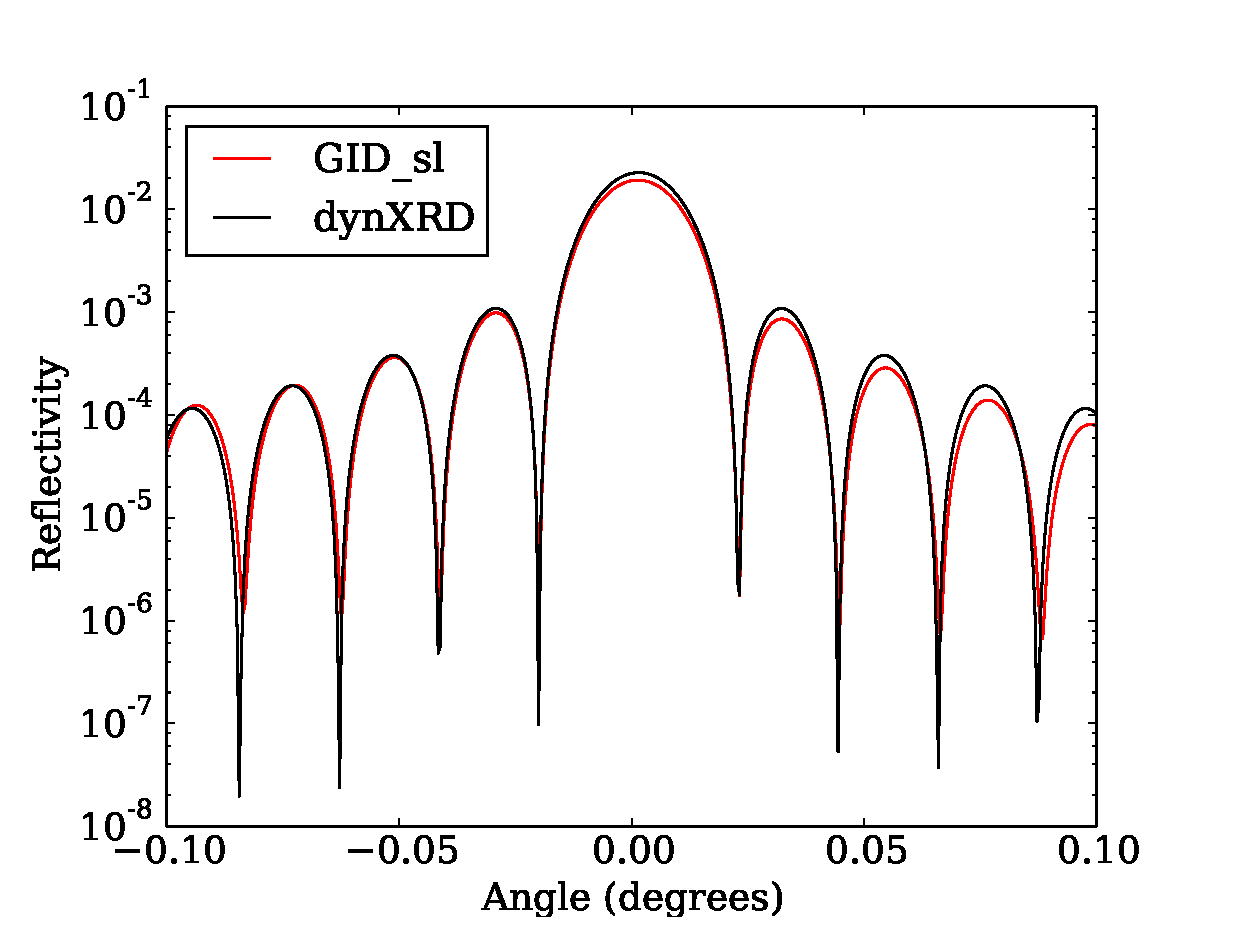
\includegraphics[width=\textwidth]{pics/test2.eps}
  \caption{Symmetric case: $v_\parallel=(1, -1, 0)$, $v_\perp=(1,1,1)$.}
  \label{test2}
 \end{subfigure}
 \begin{subfigure}[h]{0.49\textwidth}
  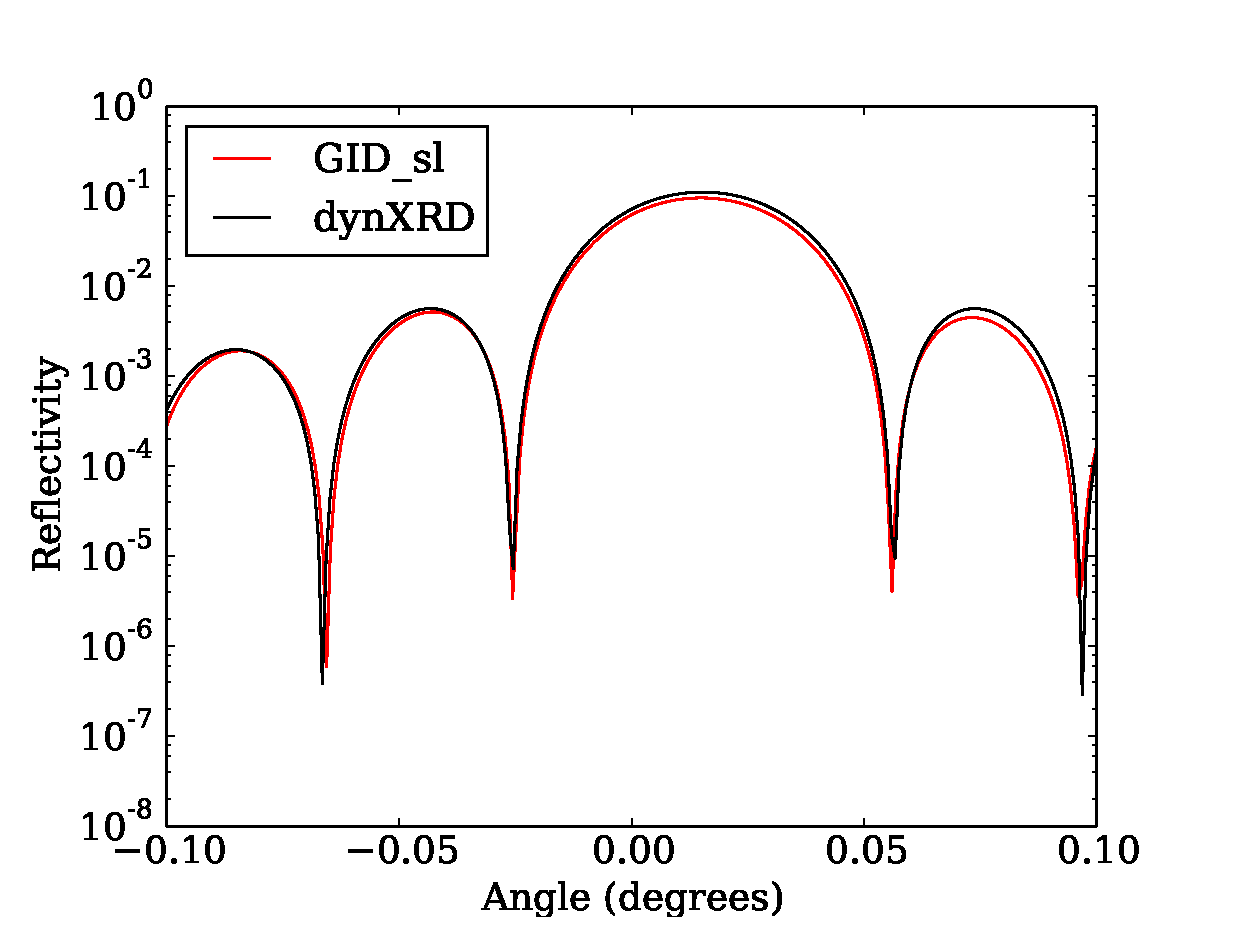
\includegraphics[width=\textwidth]{pics/test7.eps}
  \caption{Asymmetric case: $v_\parallel=(3, -2, -1)$, $v_\perp=(1,1,1)$.}
  \label{test7}
 \end{subfigure}
 \caption{$002$ reflection for a MgO layer of thickness $100\;nm$ in non-coplanar geometry.}\label{testsMgO}
\end{figure}

\begin{figure}[h]
 \centering
 \begin{subfigure}[h]{0.49\textwidth}
  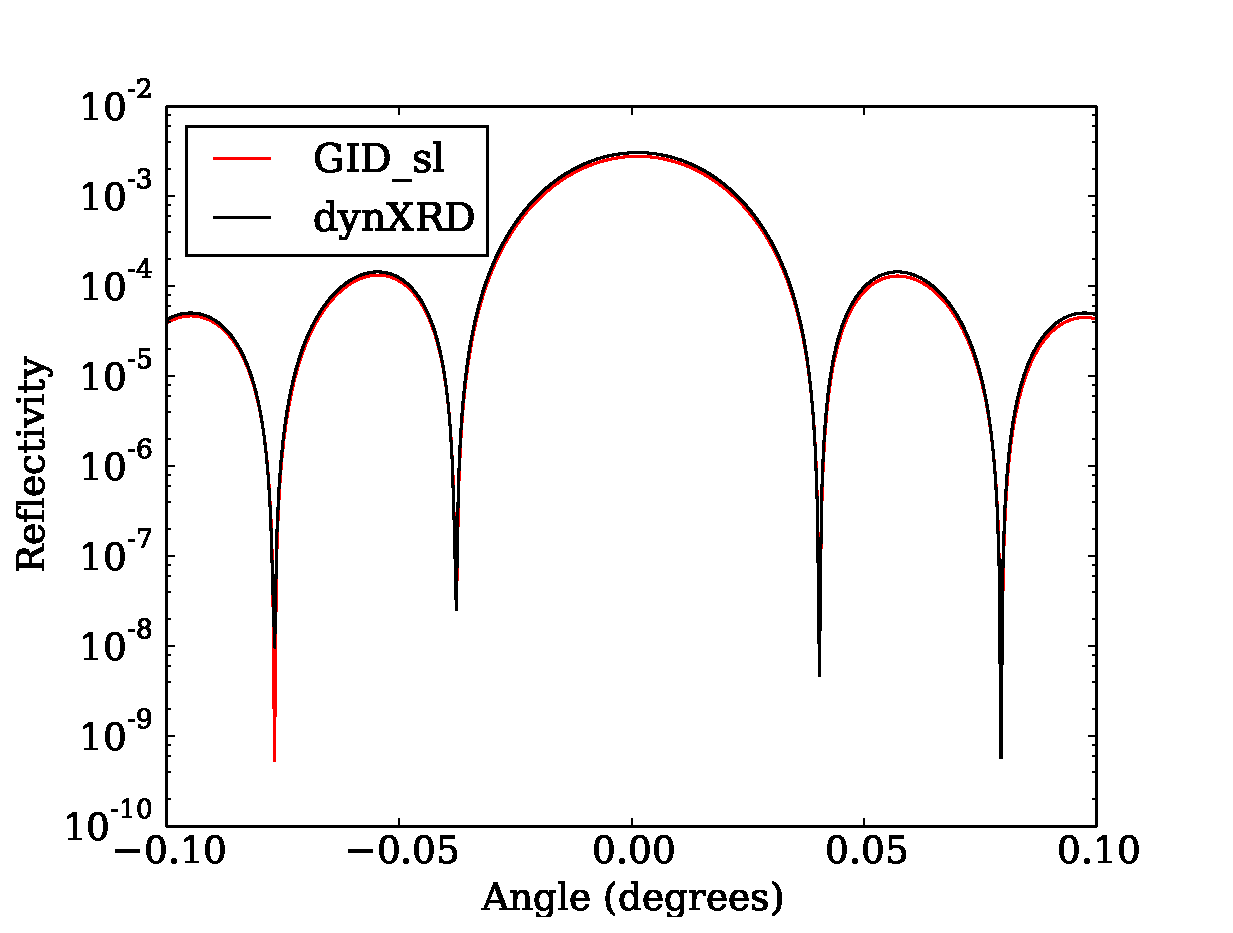
\includegraphics[width=\textwidth]{pics/test9.eps}
  \caption{Symmetric, coplanar case: $v_\parallel=(0, 0, 1)$, $v_\perp=(1,0,0)$.}
  \label{test9}
 \end{subfigure}
 \begin{subfigure}[h]{0.49\textwidth}
  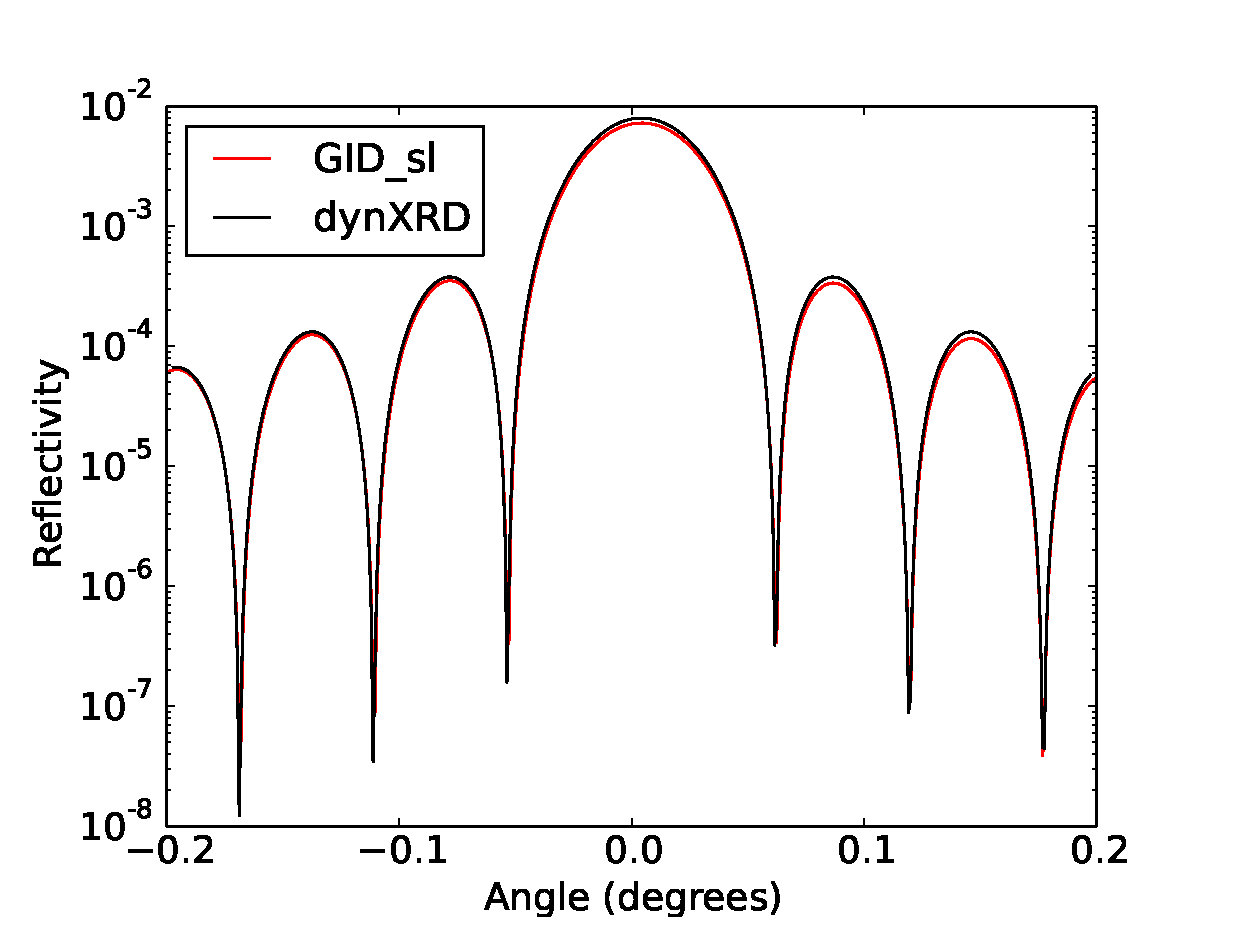
\includegraphics[width=\textwidth]{pics/test11.eps}
  \caption{Asymmetric, non-coplanar case: $v_\parallel=(-1, 1, 4)$,\newline$v_\perp=(1,1,0)$.}
  \label{test11}
 \end{subfigure}
 \caption{$300$ reflection for a LiNbO$ _3$ layer of thickness $100\;nm$.}\label{testsLiNbO3}
\end{figure}
It can be noted that simulations made with \textit{GID\_sl} and \textit{dynXRD} give analogous results in all cases even though the methods used by the programs are different.

\newpage
\subsection{Diffraction profiles of strained crystals}\label{res2}

Simulations of strained crystals are shown in figure \ref{testsstrain}. The main peak exhibits a Darwin plateau which is due to reflection from the substrate. On the other hand, smaller peaks reveal the presence of the strained layer. Both plots show a $002$ reflection with energy $10\; keV$. The substrate and the layer have the same structure and orientation. The layer is $100\; nm$ thick and has $1\%$ lattice strain.
\begin{figure}[h]
 \centering
 \begin{subfigure}[h]{0.49\textwidth}
  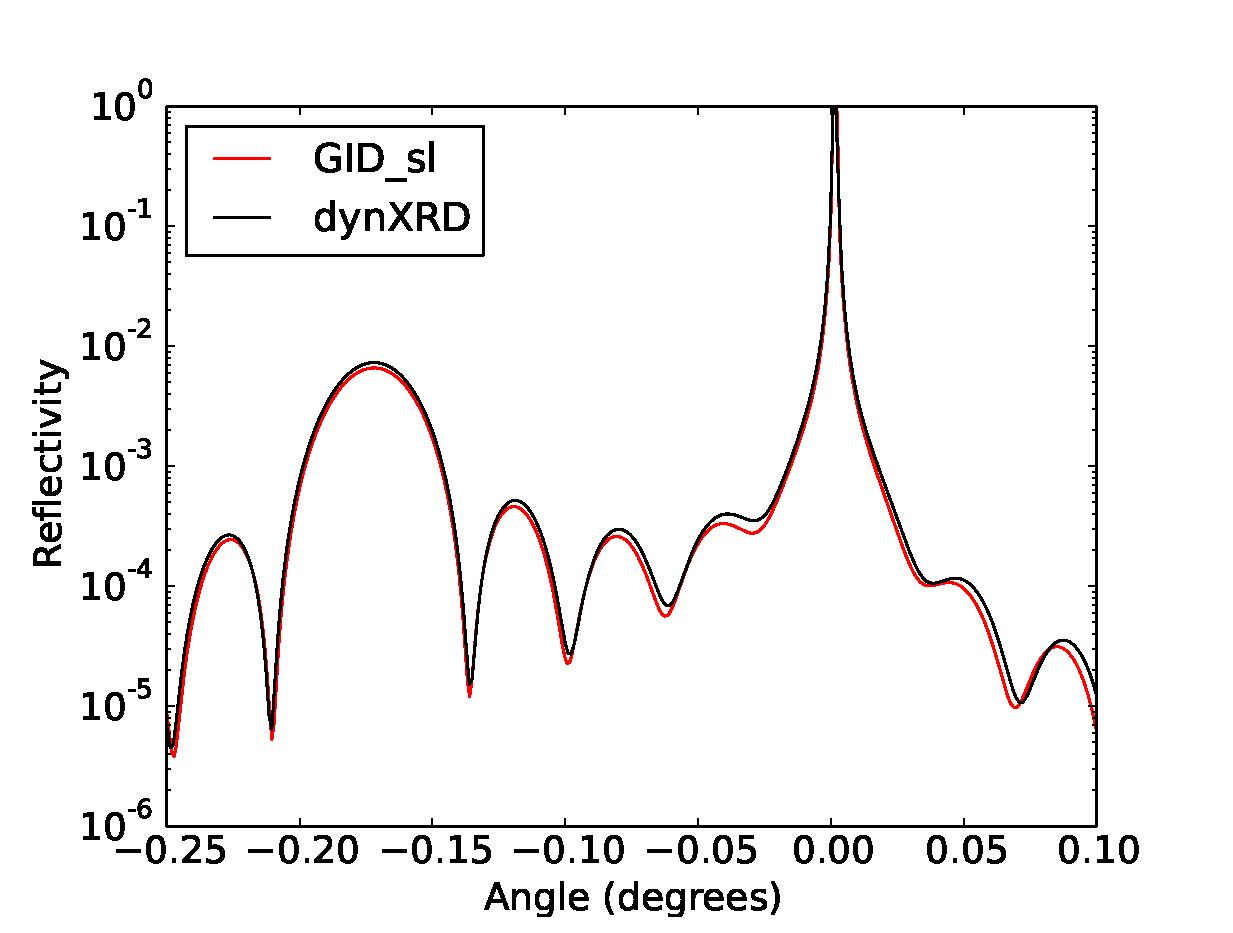
\includegraphics[width=\textwidth]{pics/test12.eps}
  \caption{MgO (cubic unit cell): symmetric, coplanar case.}\label{test12}
  \label{test12}
 \end{subfigure}
 \begin{subfigure}[h]{0.49\textwidth}
  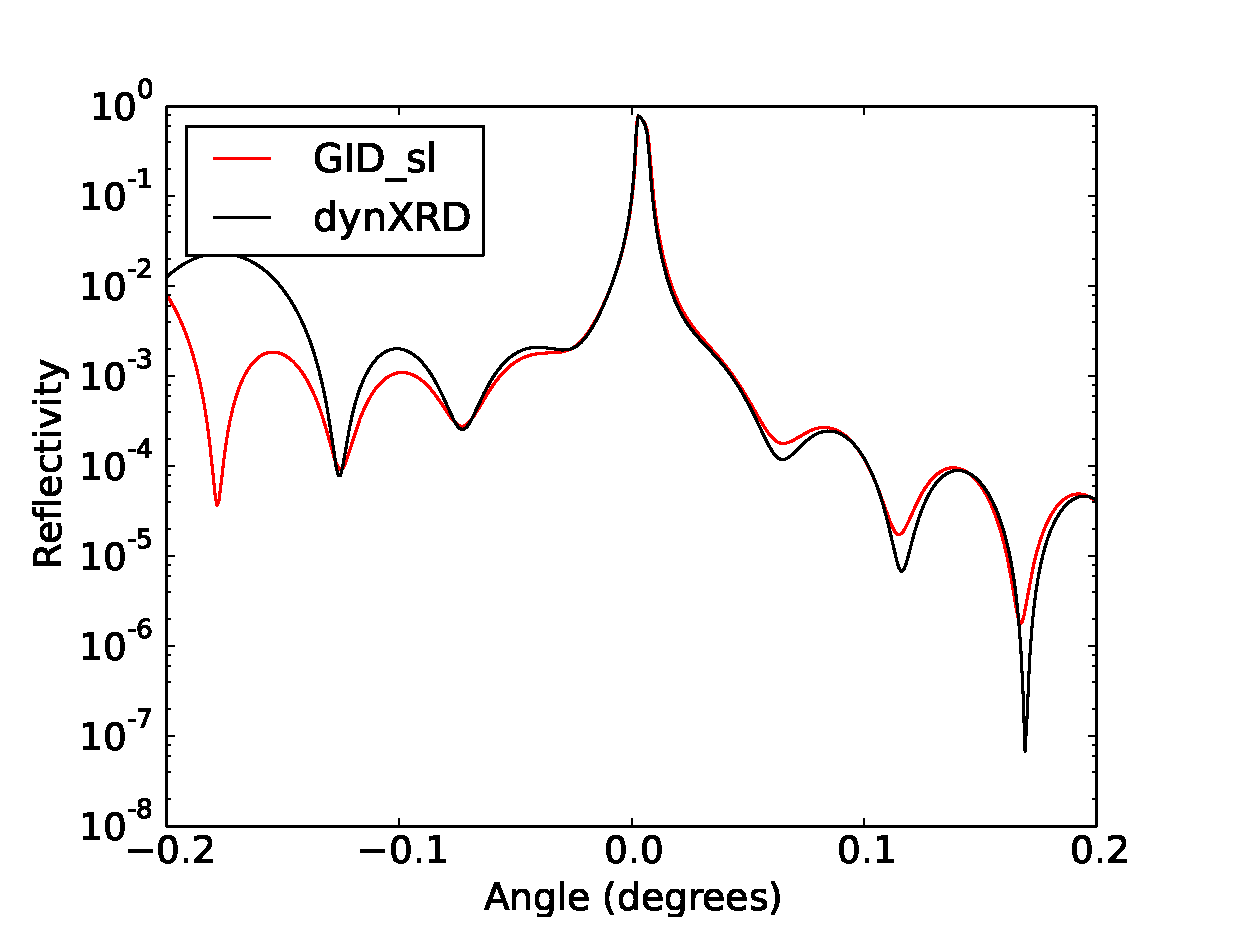
\includegraphics[width=\textwidth]{pics/test14.eps}
  \caption{BaTiO$ _3$ (tetragonal unit cell): asymmetric, non-coplanar case.}\label{test14}
  \label{test14}
 \end{subfigure}
 \caption{002 reflection for strained crystals.}\label{testsstrain}
\end{figure}


Figure \ref{GaAs_both} shows the 004 Cu $K\alpha_1$ reflection of a structure consisting of four epitaxial GaAs layers of different thickness on a GaAs substrate \cite{Bartels:a25435}. 
\begin{figure}[h]
 \centering
 \begin{subfigure}[h]{0.49\textwidth}
  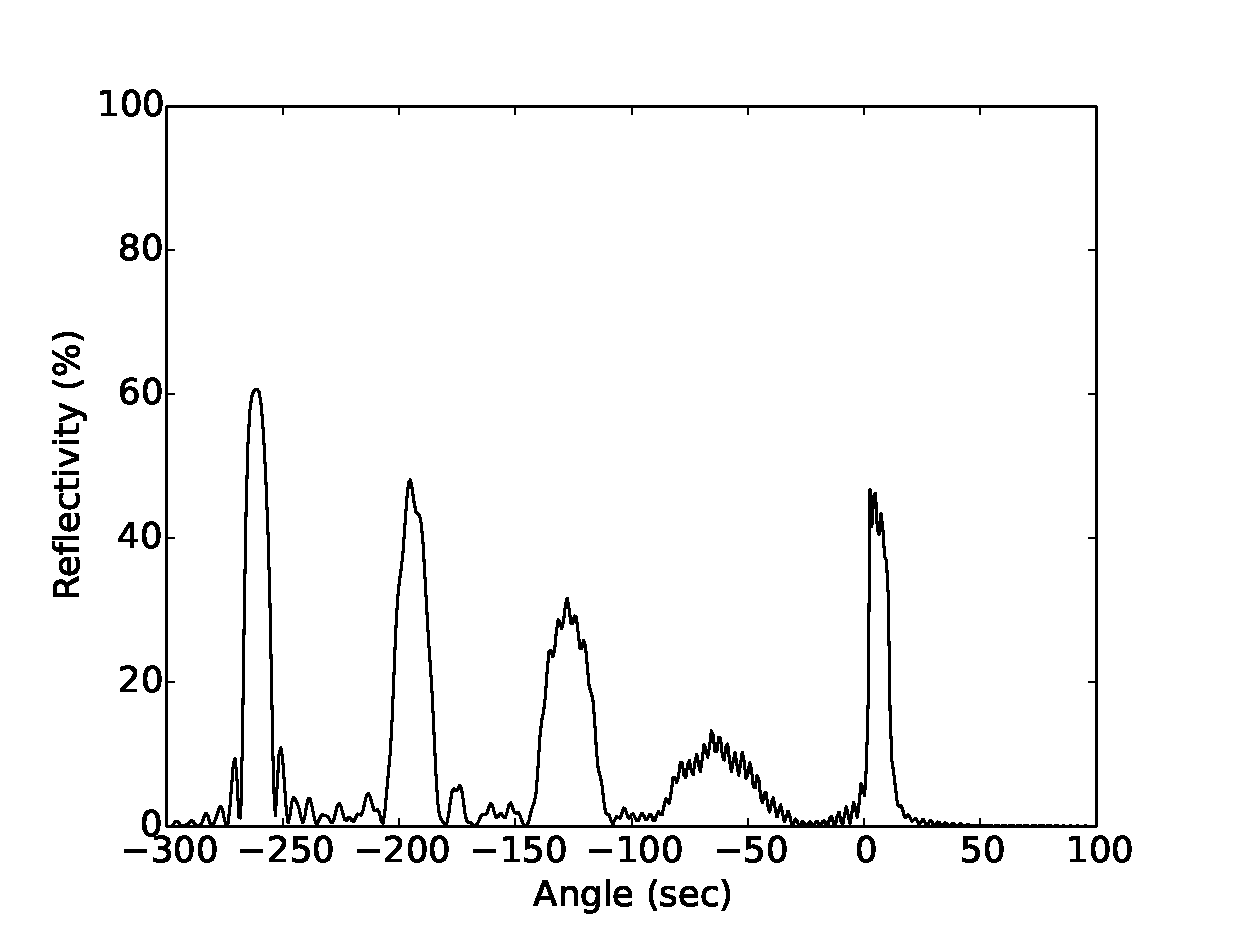
\includegraphics[width=\textwidth]{pics/GaAs.eps}
  \caption{}
  \label{GaAs}
 \end{subfigure}
 \begin{subfigure}[h]{0.50\textwidth}
  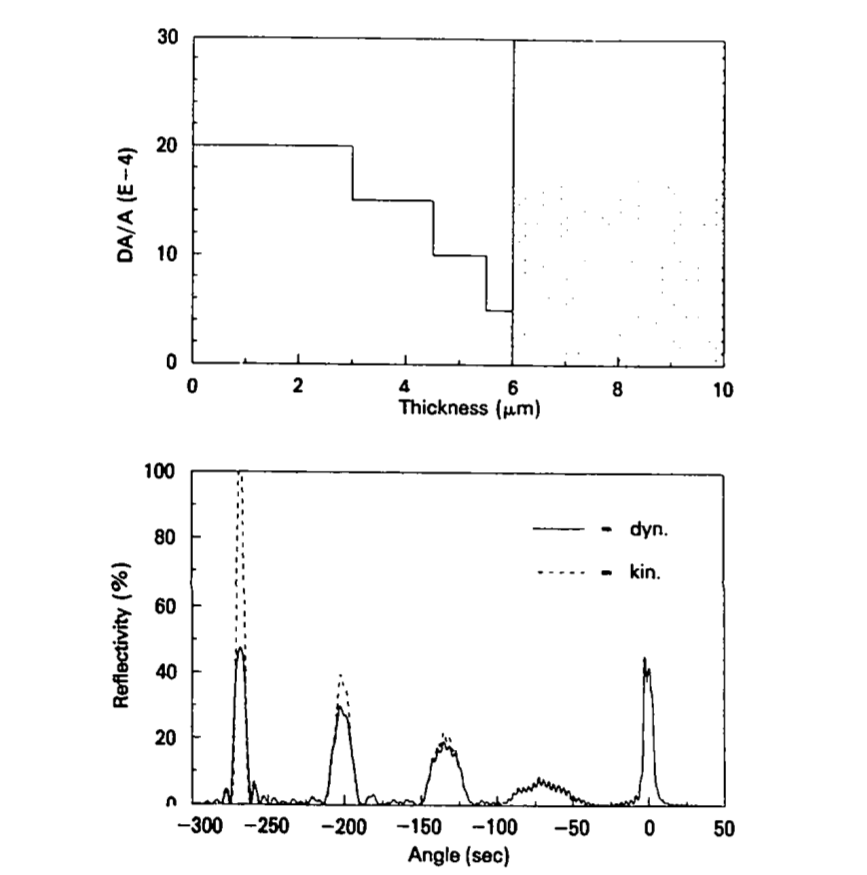
\includegraphics[width=1.2\textwidth]{pics/GaAs.png}
  \caption{}
  \label{GaAs_article}
 \end{subfigure}
 \caption{The substrate surface is taken as the origin of the thickness scale in the depth profile. The plot in figure \ref{GaAs_article} from Bartels et al. \cite{Bartels:a25435} compares diffraction profiles calculated with the dynamical and kinematical theory, while figure \ref{GaAs} shows a simulation made with \textit{dynXRD}.
}\label{GaAs_both}
\end{figure}

\subsection{Comparison with experimental data}\label{data}
The program was used to investigate the strain profile of a sample of SrTiO$ _3$. An external electric field was applied on the crystal, inducing a transition from a cubic symmetry to a tetragonal symmetry. Therefore, a model was developed assuming the following function for the strain of the $c$ parameter
\begin{equation}
 \frac{\Delta c}{c}=A e^{-x}(1+x)
\end{equation}
where $A$ is the maximum strain and $x$ is the relative depth (i.e. $x=depth/t_s$ where $t_s$ is related to the thickness of the distorted layer). Gaussian and lorenztian functions were also tested but showed lower compatibility with experimental data.
The reflectivity of the sample was measured for the $002$ reflection in a symmetric coplanar geometry ($Energy=8 keV$).
The model parameters $A$ and $t_s$ where then fitted against the measured data. Figure \ref{SrTiO3_2} shows a plot of the resulting fitting function compared to experimental data.



\begin{figure}[h]
\begin{center}
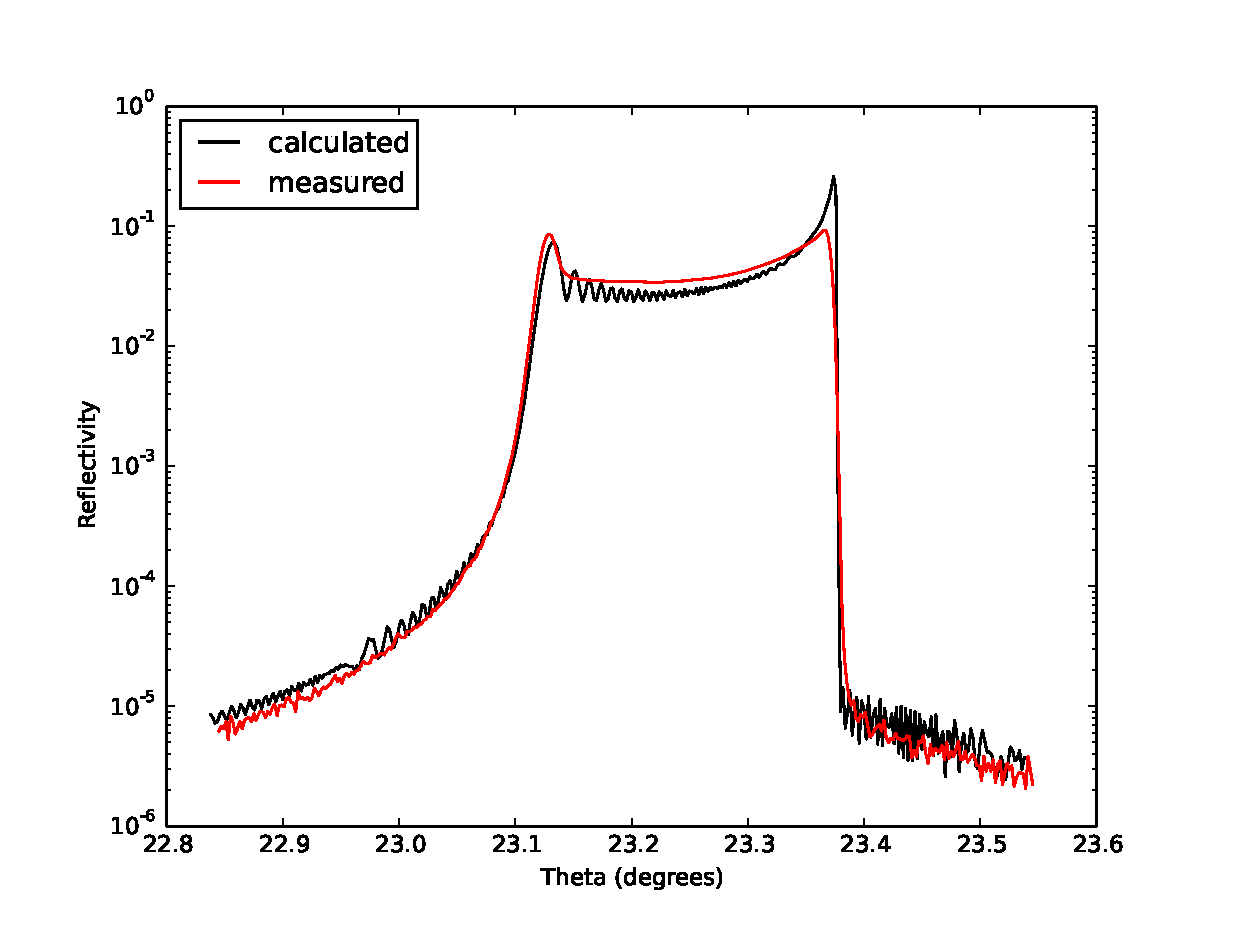
\includegraphics[width=\textwidth]{pics/SrTiO3_2.eps}
\caption{002 symmetric coplanar reflection from a strained sample of SrTiO$ _3$.}
\label{SrTiO3_2}
\end{center}
\end{figure}

The estimated values are approximately $1 \%$ for the maximum strain and $0.6 \mu m$ for the strain thickness.\\
%$A=(1.034 \pm 0.004) \%$ and $t_s=(5.93 \pm 0.06) \mu m$

% The same model was applied for fitting with different energies of the incident beam.
% 
% 
% \begin{figure}[h]
%  \centering
%  \begin{subfigure}[h]{0.49\textwidth}
%   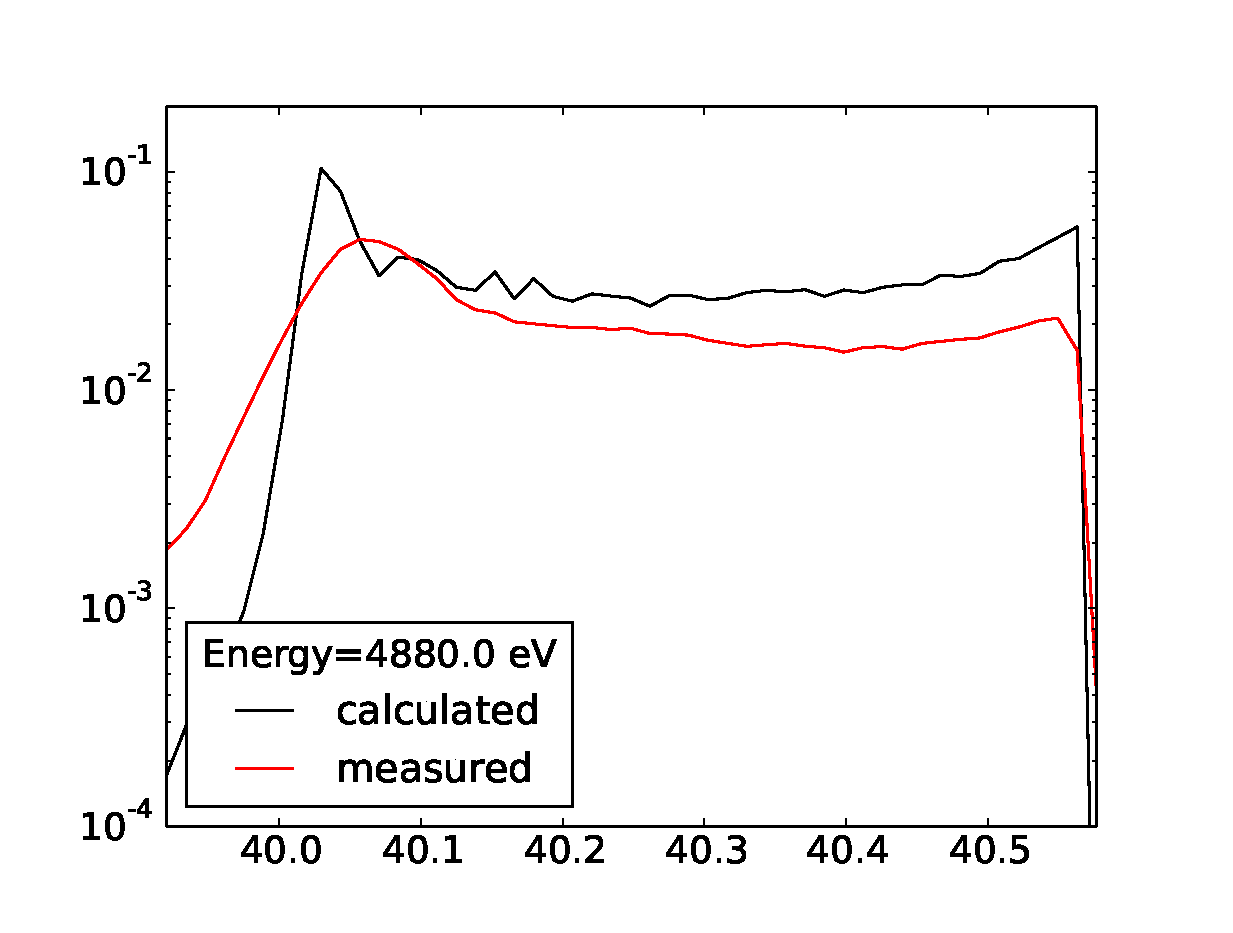
\includegraphics[width=\textwidth]{pics/SrTiO3_4880.eps}
%   \caption{}
%   \label{en1}
%  \end{subfigure}
%  \begin{subfigure}[h]{0.49\textwidth}
%   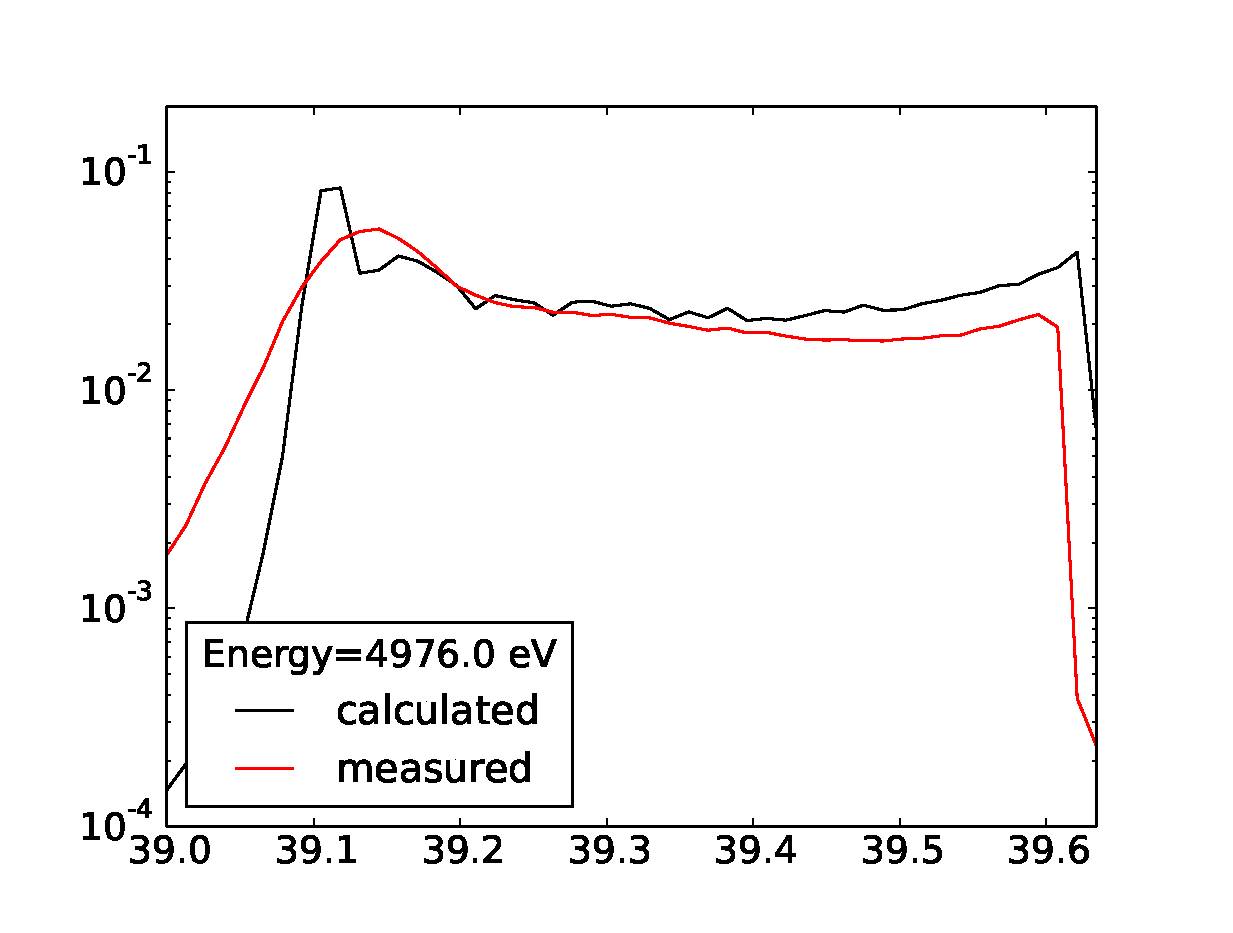
\includegraphics[width=\textwidth]{pics/SrTiO3_4976.eps}
%   \caption{}
%   \label{en2}
%  \end{subfigure}\\
%  \begin{subfigure}[h]{0.49\textwidth}
%   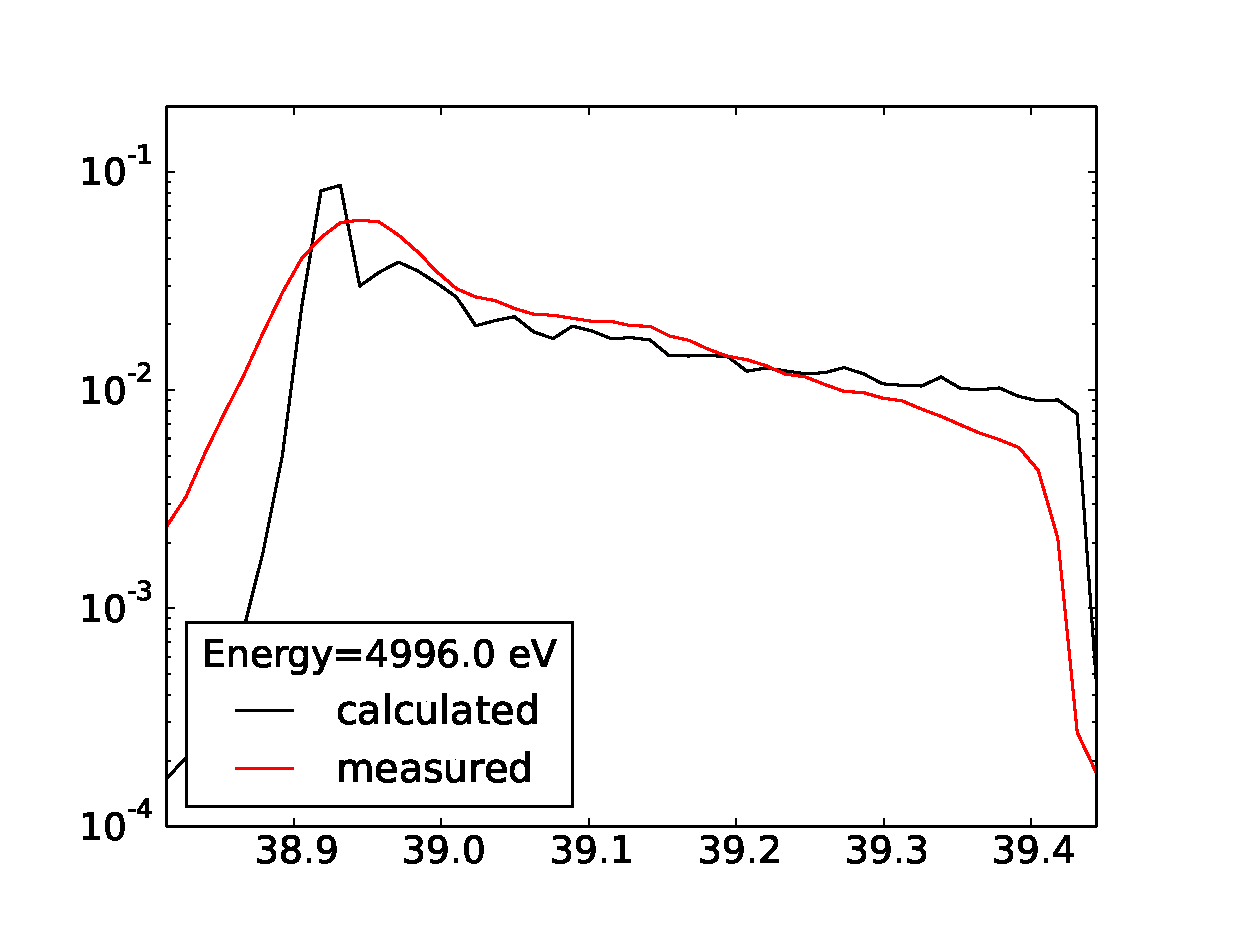
\includegraphics[width=\textwidth]{pics/SrTiO3_4996.eps}
%   \caption{}
%   \label{en3}
%  \end{subfigure}
%  \begin{subfigure}[h]{0.49\textwidth}
%   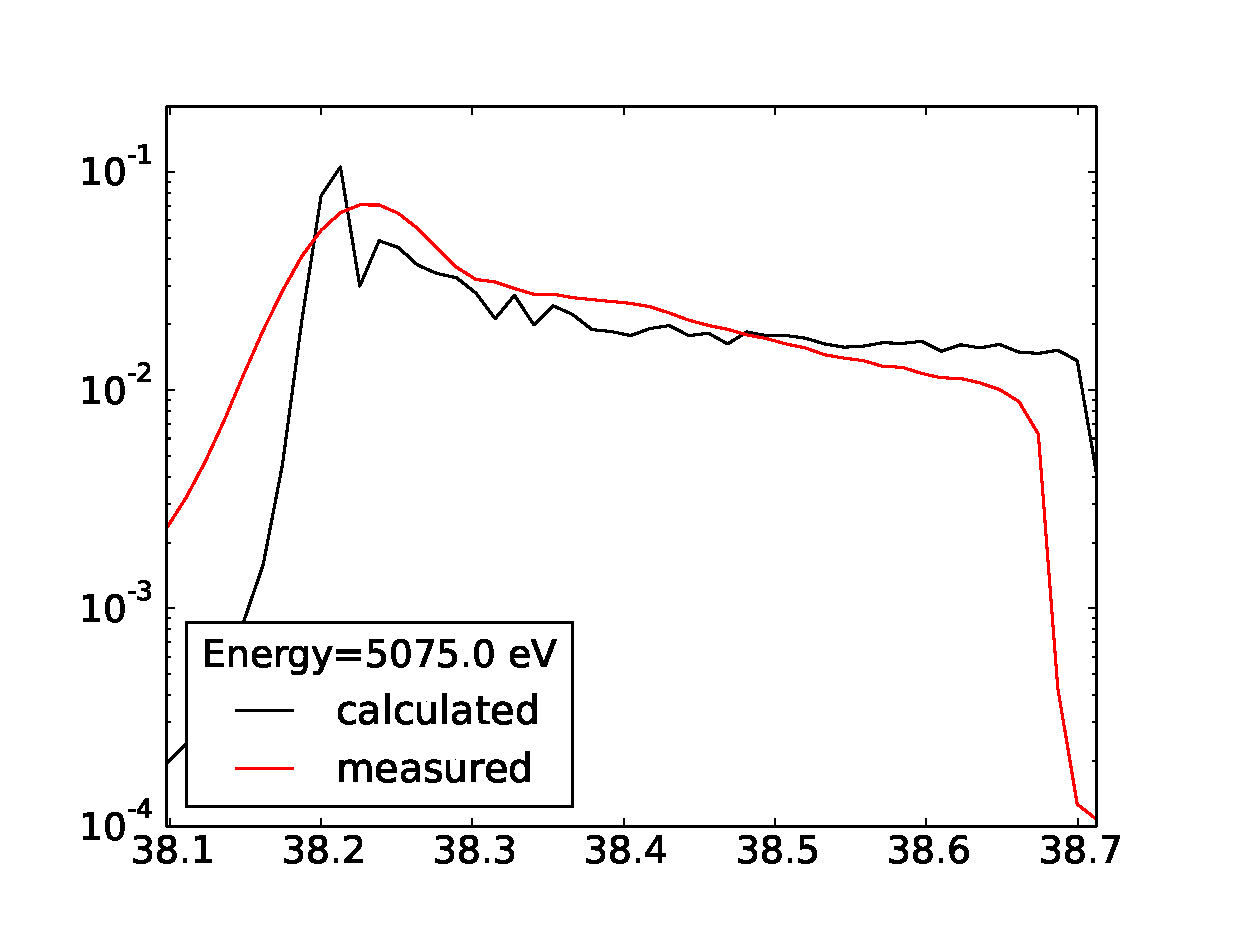
\includegraphics[width=\textwidth]{pics/SrTiO3_5075.eps}
%   \caption{}
%   \label{en4}
%  \end{subfigure}
%  \caption{}\label{en}
% \end{figure}

\clearpage 



\nocite{*}
\bibliographystyle{unsrt} 
\addcontentsline{toc}{section}{References}
\bibliography{Elements_of_Modern_X_ray_Physics,X_ray_Diffraction,bartels,Dynamical_Scattering_of_X_rays_in_Crysta}{}



\end{document}
